\chapter{Spatial and Temporal Patterns: CNNs and LSTMs}

The Earth’s atmosphere is a multi-dimensional, spatiotemporal continuum where the state of any given air parcel is inextricably linked to its immediate neighbors and its historical trajectory. Capturing the complex dynamics of this system—ranging from the localized turbulence of a convective cell to the global-scale oscillations of the planetary waves—requires mathematical architectures that inherently respect the geometry of space and the continuity of time. This chapter examines the transition from point-based neural processing to architectures that leverage the physical principles of local correlation and temporal persistence, specifically Convolutional Neural Networks (CNNs) and Long Short-Term Memory (LSTM) networks. These models serve as the structural backbone for modern weather emulators, providing the high-dimensional "eyes" and "memory" necessary to track the pulse of the planetary fluid.

\section{The Geometry of Grid Data: Exploiting Local Correlation}

The fundamental limitation of the Multi-Layer Perceptrons (MLPs) discussed in Chapter 4 is their requirement to "flatten" data into a one-dimensional vector. In the context of global atmospheric grids, such as those provided by the ERA5 reanalysis or high-resolution satellite imagery, flattening is a mathematical rejection of physical reality. When a 2D map of geopotential height is converted into a 1D list, the spatial proximity of the points is destroyed; a grid cell in New York is suddenly separated from its neighbor in New Jersey by thousands of indices in the vector. To a standard MLP, the atmosphere possesses no inherent "shape," only a sequence of independent numbers. This structural blindness prevents the model from learning the fundamental derivative relationships—the gradients and Laplacians—that define fluid dynamics (Goodfellow et al., 2016).

Atmospheric processes are defined by the principle of \textbf{Local Correlation}: the physical state at any coordinate $(x, y, z)$ is strongly constrained by the state of its immediate neighbors through the processes of diffusion, advection, and pressure-gradient forcing. To capture this physics, weather data must be treated as a \textbf{Tensor}—a multi-dimensional array that preserves topological relationships. A standard global grid is typically a 3D tensor with dimensions of $(Latitude, Longitude, Channels)$, where channels represent different physical variables such as temperature, wind, and humidity. By utilizing architectures that operate directly on these tensors, we ensure that the model "sees" the atmosphere as a continuous, rotating fluid rather than a collection of isolated points. 

\begin{figure}[H]
    \centering
    \dummygraphic{Figure Placeholder}
    \caption{The geometry of meteorological data. Unlike MLPs which flatten grids, CNNs utilize tensors to preserve spatial connectivity, enabling the model to capture local correlations essential for fluid advection.}
    \label{fig:tensor_geometry}
\end{figure}

\section{The Convolutional Stencil: Learning the Eyes of the Storm}

The origin of the Convolutional Neural Network (CNN) lies in the study of the biological visual cortex. This inspired the development of "digital eyes" that recognize patterns by breaking them down into a hierarchy of increasingly complex structures. In meteorology, a CNN acts as a sophisticated \textbf{Digital Stencil} that sweeps across the global atmospheric tensor, identifying the specific physical signatures of weather. 

The mathematical operation that defines this spatial vision is the \textbf{Convolution}. For an input weather grid ($I$) and a small set of learned weights known as a kernel ($K$), the output feature map ($O$) is calculated by sliding the kernel over the grid:

\begin{equation}
(I * K)(i, j) = \sum_{m} \sum_{n} I(i + m, j + n) K(m, n)
\end{equation}

Each kernel is effectively a "Physical Question" the network asks the data. A kernel might ask: "Is there a sharp zonal gradient in pressure at this location?" By stacking multiple layers, the network builds a physical hierarchy: the first layer detects simple gradients; middle layers combine these into frontal zones; and final layers recognize fully-formed cyclonic vortices.

\begin{table}[H]
\centering
\caption{Hierarchical Feature Extraction in Atmospheric CNNs}
\begin{tabular}{|l|l|p{8cm}|}
\hline
\textbf{Layer Depth} & \textbf{Feature Scale} & \textbf{Learned Patterns} \\ \hline
Shallow & Local & Temperature gradients, humidity spikes, cloud edges. \\ \hline
Middle & Mesoscale & Squall lines, sea-breeze fronts, gravity waves. \\ \hline
Deep & Synoptic & Extra-tropical cyclones, Jet stream ripples, blocking highs. \\ \hline
Global & Planetary & Rossby wave packets, moisture conveyors, teleconnections. \\ \hline
\end{tabular}
\end{table}

\section{Time Series and the Failure of the Markov Assumption}

While CNNs capture the "Where" of weather, prediction is a problem of "When." The atmosphere is a continuous stream of energy where the future is deeply linked to the past. This is the concept of \textbf{Atmospheric Memory}. In simple statistical models, we often invoke the \textbf{Markov Assumption}:

\begin{equation}
P(X_{t+1} | X_t, X_{t-1}, \dots, X_0) = P(X_{t+1} | X_t)
\end{equation}

However, the Earth system is profoundly \textbf{Non-Markovian}. The state is influenced by "Hidden Variables" with long temporal scales, such as soil moisture or ocean heat content. To predict the weather a month from now, one must know the history of the ENSO cycle or the MJO. This reservoir of information is represented by the \textbf{Hidden State} of a recurrent network, allowing the AI to track slow signals in a chaotic system.

\section{Long Short-Term Memory (LSTM): Gating the Planetary Pulse}

The breakthrough for capturing multi-scale temporal signals was the \textbf{Long Short-Term Memory (LSTM)} network (Hochreiter \& Schmidhuber, 1997). LSTMs solve the \textbf{Vanishing Gradient} problem by introducing a \textbf{Cell State} ($C_t$) and a series of \textbf{Gates}.

The gating mechanism acts as a set of digital valves. For a given time step $t$, the network calculates the Forget Gate ($f_t$), Input Gate ($i_t$), and Output Gate ($o_t$):

\begin{equation}
f_t = \sigma(W_f [h_{t-1}, x_t] + b_f)
\end{equation}
\begin{equation}
i_t = \sigma(W_i [h_{t-1}, x_t] + b_i)
\end{equation}
\begin{equation}
C_t = f_t * C_{t-1} + i_t * \tanh(W_c [h_{t-1}, x_t] + b_c)
\end{equation}

\begin{figure}[H]
\centering
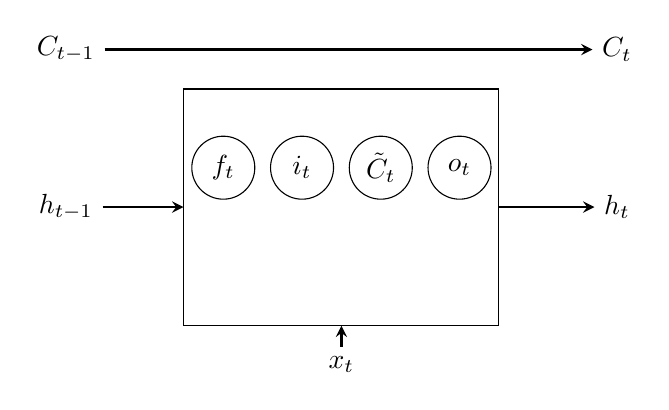
\begin{tikzpicture}[
    cell/.style={rectangle, draw, minimum width=4cm, minimum height=3cm},
    gate/.style={circle, draw, minimum size=0.8cm, inner sep=0pt},
    arrow/.style={thick,->,>=stealth}
]
    % Cell Box
    \node (cbox) [cell] {};
    
    % Gates
    \node (f) [gate, above of=cbox, yshift=-0.5cm, xshift=-1.5cm] {$f_t$};
    \node (i) [gate, above of=cbox, yshift=-0.5cm, xshift=-0.5cm] {$i_t$};
    \node (ct) [gate, above of=cbox, yshift=-0.5cm, xshift=0.5cm] {$\tilde{C}_t$};
    \node (o) [gate, above of=cbox, yshift=-0.5cm, xshift=1.5cm] {$o_t$};
    
    % Flow
    \node (h_prev) [left of=cbox, xshift=-2.5cm] {$h_{t-1}$};
    \node (x_curr) [below of=cbox, yshift=-1cm] {$x_t$};
    \node (c_prev) [above of=cbox, yshift=1cm, xshift=-3.5cm] {$C_{t-1}$};
    \node (c_curr) [above of=cbox, yshift=1cm, xshift=3.5cm] {$C_t$};
    \node (h_curr) [right of=cbox, xshift=2.5cm] {$h_t$};

    \draw [arrow] (h_prev) -- (cbox.west);
    \draw [arrow] (x_curr) -- (cbox.south);
    \draw [arrow] (c_prev) -- (c_curr);
    \draw [arrow] (cbox.east) -- (h_curr);
\end{tikzpicture}
\caption{Schematic of an LSTM Cell. The forget gate ($f_t$) controls the preservation of long-term atmospheric signals, while the input gate ($i_t$) and output gate ($o_t$) modulate the influence of new observations.}
\label{fig:lstm_tikz}
\end{figure}

The forget gate $f_t$ decides how much historical memory to keep, while the input gate $i_t$ decides how much new information to add. This allows a physical signal—like a moisture plume—to be carried across hundreds of steps without degradation.

\section{Operational Reality: 3D Convolutions and VRAM Bottlenecks}

The atmosphere is volumetric. To capture its 3D dynamics (e.g., vertical tilt of a wave), we must employ \textbf{3D Convolutions} treating height as a spatial dimension. This transforms data from pixels to \textbf{Voxels}. 

However, the memory footprint scales as $\mathcal{O}(D \times H \times W \times C \times K^3)$. This cubic growth quickly saturates available \textbf{Video Random Access Memory (VRAM)}, earning 3D CNNs the reputation of "VRAM Killers." 

\begin{infobox}
\textbf{Case Study: Superstorm Sandy's 3D Core}\\
In Sandy (2012), the vertical structure was the deciding factor. The interaction between the tropical cyclone and a deep upper-level trough created "Vertical Synchronization." A 2D model would miss this; a 3D CNN identifies the phase alignment that pumped massive latent heat out of the Gulf Stream.
\end{infobox}

\section{Summary: Spatiotemporal Fusion}

Integration of CNNs and LSTMs creates "Digital Synoptic Meteorologists." While powerful, the "Sequential Bottleneck" of LSTMs and the "VRAM Barrier" of 3D CNNs indicate we are reaching the limits of localized architectures. The following chapters explore the \textbf{Transformer Revolution}, providing a way to see the entire globe at once via "Attention."

\section*{Bibliography}
\begin{itemize}
    \item Goodfellow, I., et al. (2016). \textit{Deep Learning}. MIT Press.
    \item Hochreiter, S., \& Schmidhuber, J. (1997). Long short-term memory. \textit{Neural Computation}.
    \item LeCun, Y., et al. (1998). Gradient-based learning applied to document recognition. \textit{Proceedings of the IEEE}.
    \item Shi, X., et al. (2015). Convolutional LSTM network: A machine learning approach for precipitation nowcasting. \textit{NIPS}.
\end{itemize}
